\documentclass[12pt
,a4paper
,titlepage
%,twoside
,openany % ouvre les sections indifféremment sur la page de gauche ou de droite
]{book}

% Paramétrages de la langue et de l'encodage
\usepackage[utf8]{inputenc}
\usepackage{textcomp}
\usepackage[french]{babel}
\usepackage[T1]{fontenc}

% formules mathématiques
\usepackage{amsmath}
\usepackage{amsfonts}
\usepackage{amssymb}

% gestion des graphiques
\usepackage{graphicx}
% positionnement flottant des graphiques
\usepackage{float}
% Gestion des couleurs
\usepackage[usenames,dvipsnames]{xcolor}

% Redefinition des liens web
\usepackage{url}
\usepackage[colorlinks=false,urlbordercolor=white,linkbordercolor=white]{hyperref}

\usepackage{longtable}
\usepackage{array}

% Définition des marges de la page
\usepackage[left=2cm,right=2cm,top=2cm,bottom=2cm]{geometry}

% Polices de caractères
\usepackage{lmodern}
\usepackage{mathptmx} % times, y compris dans les formules mathématiques

% Insertion de code source dans le texte, à utiliser avec \begin{lstlisting} et \lstset{java|html|php...}
\usepackage{listings}
\lstset{ %
basicstyle=\small\ttfamily, %
breaklines=true, %
columns=spaceflexible, %
}

% Définition des entêtes
\usepackage{fancyhdr}
\pagestyle{fancy}

% Redéfinition des titres de section
\usepackage{titlesec}

% Insertion de graphiques à des emplacements définis
\usepackage[abs]{overpic}

% règles typographiques de l'Imprimerie nationale
\usepackage[all]{nowidow}
\usepackage[
% frenchchapters renomme le premier chapitre, mais :
%	- cela pose problème dans la table des matières
%	- cela ne peut être utilisé qu'avec la renumérotation des chapitres activée
%frenchchapters,
parindent,
lastparline,
hyphenation
]{impnattypo}

% Renumérotation des chapitres
%\renewcommand{\thesection}{\Alph{section})}
%\renewcommand{\thesubsection}{\arabic{subsection} -}
%\renewcommand{\thesubsubsection}{\alph{subsubsection} -}
%\usepackage{engrec}
%\renewcommand{\theparagraph}{\engrec{paragraph})}
%\setcounter{secnumdepth}{4}

% Génération du code Ipsum lorem
%\usepackage{blindtext}


% Definition des couleurs IRSTEA
\definecolor{titreColor}{RGB}{0,58,128}  % Marine
\definecolor{stitreColor}{RGB}{0,158,224}  % Ocean
\definecolor{auteurColor}{RGB}{0,58,128}     % Marine
\definecolor{texteColor}{RGB}{164,196,0}     % Prairie

% Definition des chapitres
\titleformat{\chapter}[display]
{\normalfont\Large\filcenter\sffamily}
%{\titlerule[1pt]%
% \vspace{1pt}%
% \titlerule
% \vspace{1pc}%
{
 \Large\color{titreColor}{
 %\MakeUppercase{\chaptertitlename}
 \chaptertitlename~\thechapter}
 }
{1pc}
%{\titlerule
%% \vspace{1pc}%
 \Huge

\titleformat{\section}[block]
{\color{titreColor}\normalfont\Large\bfseries\sffamily}
{\color{titreColor}\thesection}{1em}{}

\titleformat{\subsection}[block]
{\color{stitreColor}\bfseries\sffamily}
{\color{stitreColor}\thesubsection}{1em}{}

\titleformat{\subsubsection}[block]
{\color{stitreColor}\sffamily\em}
{\color{stitreColor}{\thesubsection}}{1em}{}

% Bibliographie
% natbib est indispensable si la biblio contient des accents
% Options pour natbib (extrait de http://merkel.zoneo.net/Latex/natbib.php)
%    round: (par défaut) pour des parenthèses arondies (());
%    square: pour des crochets ([]);
%    curly: pour des accolades ({});
%    angle: pour des équerres (<>) ;
%    colon: (par défaut) pour séparer les citations multiples par deux points (:);
%    comma: pour utiliser une virgule comme séparateur;
%    authoryear: (par défaut) pour des citations auteurs-année;
%    numbers: pour des citations numériques;
%    super: pour des citations numériques en exposant, comme dans Nature;
%    sort: ordonne les citations multiples dans l'ordre dans lequel elles apparaissent dans la bibliographie;
%    sort&compress: comme sort mais en plus les citations numériques multiples sont comprimées, si possible (3-6, 15, par exemple);
%    longnamesfirst: transforme la première citation à une référence en une version étoilée (avec la liste complète des auteurs) et le citations suivantes normales (liste abbrégée);
%    sectionbib: pour redéfinir \thebibliography pour avoir une \section* à la place d'un \chapter*; valide seulement pour les classes de document possédant la commande \chapter; à utiliser avec le paquetage  chapterbib;
%    nonamebreak: garde tous les noms d'auteurs d'une citation sur une même ligne; celà cause des problèmes de débordement, mais permet de résoudre certains problèmes liés à hyperref.

% En cas de souci, supprimez les fichiers .aux et .bbi après modification des paramètres
\usepackage[square,sort,comma,numbers]{natbib}
% styles natbib natifs : abbrvnat, plainnat, unsrtnat
\bibliographystyle{plainnat}
\usepackage{hypernat}
% Ajout de la référence à la bibliographie dans la table des matières
\usepackage[nottoc, notlof, notlot]{tocbibind}

%Données de titre et d'auteur pour la page de garde
\newcommand{\titre}{Logiciel Filo-Science}
\newcommand{\sousTitre}{Manuel d'installation et de paramétrage}
\newcommand{\auteur}{Éric Quinton}
\newcommand{\dateModif}{15/11/2019 - v1.3.0}
\usepackage[final]{pdfpages} 

\usepackage{lscape}
\usepackage[font=small,labelfont=bf]{caption}

\begin{document}
%Supprime les veuves et orphelines
\widowpenalty=10000
\clubpenalty=10000
\raggedbottom 

% Integrer la page de garde
%\setcounter{page}{0}
\thispagestyle{empty}
% Logo IRSTEA
\vspace{-2cm}
\hspace{-2cm}

\includegraphics[width=3.06cm,height=3.06cm,keepaspectratio]{logo_irstea}%


\vspace*{4cm}
\hspace{5cm}
\setlength\unitlength{1mm}
% Logo de titre
\begin{overpic}[width=9.44cm,height=9.57cm,keepaspectratio]{logo_fond_droite.png}
% Titre du document
\put(-50,50){
\begin{minipage}{0.7\linewidth}
\Huge\flushright \color{titreColor}{\bfseries\sffamily\titre{}}\\
% sous-titre du document
\color{stitreColor}{\Large \bfseries\sffamily\sousTitre{}}
\end{minipage}
}
\end{overpic}

%  date et auteur
% creation de l'espace a gauche
\vspace*{1cm}
\begin{minipage}{0.5\linewidth}
\hfill
\end{minipage}
% positionnement
\begin{minipage}{0.5\linewidth}\flushleft{
% Date
\textcolor{auteurColor}{\Large\sffamily\dateModif{}}\\
\vspace*{0.1cm}
% Auteur
\textcolor{auteurColor}{\Large\sffamily\auteur{}}\\
\vspace{0.5cm}
% Adresse
\textcolor{texteColor}{\sffamily\textbf{IRSTEA} - Centre de Bordeaux\\
50, avenue de Verdun, Gazinet\\
33612 CESTAS Cedex }
}
\end{minipage}
% Ligne de logos
\begin{minipage}{\linewidth}

% logos complémentaires
%\vspace{3cm}
%\hspace{2cm}
%\includegraphics[width=3cm,height=3cm,keepaspectratio]
%{emplacement_logo}%
%\vspace{-1cm}
%\hspace{1cm}
%\includegraphics[width=3cm,height=3cm,keepaspectratio]
%{emplacement_logo}%
%\vspace{-1cm}
%\hspace{1cm}
%\includegraphics[width=3cm,height=3cm,keepaspectratio]
%{emplacement_logo}%
\end{minipage}
% Définition des entêtes
\fancyhead{}
\fancyhead[CO]{\leftmark\sffamily}
\fancyhead[CE]{ \sffamily\titre{}}
\fancyfoot[CO]{\sffamily\thepage}
\fancyfoot[CE]{\sffamily\thepage}
% Redéfinition de \cleardoublepage pour créer une page totalement vide
\makeatletter
\def\cleardoublepage{\clearpage\if@twoside \ifodd\c@page\else
  \hbox{}
  \vspace*{\fill}

  \vspace{\fill}
  \thispagestyle{empty}
  \newpage
  \if@twocolumn\hbox{}\newpage\fi\fi\fi}
\makeatother

% \cleardoublepage permet de générer une page vide 
% si le chapitre ne commence pas sur la page de droite

% Ajout d'un préambule
\frontmatter
\cleardoublepage

% Table des matières
\tableofcontents


% Début réel du texte
\mainmatter
%\cleardoublepage

\chapter{Le logiciel Filo-Science}
\section{Présentation}

Le logiciel Filo-Science a été conçu pour permettre l'enregistrement des informations concernant les poissons capturés lors des opérations de pêches scientifiques (pêches électriques, pêches au filet). 

Il a été conçu pour l'unité de recherche \textit{Écosystèmes aquatiques et changements globaux} d'IRSTEA, à Cestas (33).

Il a été écrit en PHP, les pages web sont générées en HTML et Javascript avec le composant Smarty.

\section{Fonctionnalités générales}

L'application est organisée autour de la notion de projet : un projet peut regrouper plusieurs campagnes, qui sont menées en réalisant des opérations de pêche. Les droits d'accès sont attribués par projet.

\section{Technologie employée}
\subsection{Base de données}

L'application a été conçue pour fonctionner avec Postgresql, en version 9.6. 

\subsection{Langage de développement et framework utilisé}
Le logiciel a été écrit en PHP, en s'appuyant sur le framework \textit{Prototypephp} \cite{prototypephp}, développé parallèlement par l'auteur du logiciel.

Il utilise la classe \textit{Smarty} \cite{smarty} pour gérer l'affichage des pages HTML. Celles-ci sont générées en utilisant \textit{Jquery} \cite{jquery}  et divers composants associés. Le rendu général est réalisé avec \textit{Bootstrap} \cite{bootstrap}.



\subsection{Liste des composants externes utilisés}
% \usepackage{array} is required
\begin{longtable}{|>{\raggedright\arraybackslash}p{3cm}|c|c|>{\raggedright\arraybackslash}p{3cm}|>{\raggedright\arraybackslash}p{3cm}|}
\hline 
\textbf{Nom} & \textbf{Version} & \textbf{Licence} & \textbf{Usage} & \textbf{Site} \\ 
\hline 
\endhead
PrototypePHP & 5/4/2019 & LGPL & Framework & \href{https://github.com/equinton/prototypephp}{github.com/ equinton/ prototypephp} \\ 
\hline 
Smarty & 3.1 & LGPL & Générateur de pages HTML & \href{http://www.smarty.net}{www.smarty.net} \\ 
\hline 
Smarty-gettext & 1.2.0 & LGPL & Gestion du multi-linguisme avec Smarty & \href{https://github.com/smarty-gettext/smarty-gettext}{https://github.com/smarty-gettext/smarty-gettext} \\
\hline
PHPCAS & 1.3.5 & Apache 2.0 & Identification auprès d'un serveur CAS & \href{https://wiki.jasig.org/display/CASC/phpCAS}{wiki.jasig.org/ display/ CASC/ phpCAS} \\ 
\hline 
Bootstrap & 3.3.7 & MIT & Présentation HTML & \href{http://getbootstrap.com}{get.bootstrap.com} \\ 
\hline 
js-cookie-master & 2.1.4 & MIT & Gestion des cookies dans le navigateur & \href{https://github.com/js-cookie/js-cookie}{github.com/ js-cookie/ js-cookie} \\ 
\hline 
Datatables & 1.10.15 & MIT & Affichage des tableaux HTML & \href{http://www.datatables.net/}{www.datatables. net} \\ 
\hline 
Datetime-moment &  & MIT & Formatage des dates dans les tableaux & \href{https://datatables.net/plug-ins/sorting/datetime-moment}{datatables.net/ plug-ins/ sorting/ datetime-moment} \\ 
\hline 
Moment & 2.8.4 & MIT & Composant utilisé par datetime-moment & \href{http://momentjs.com} {momentjs.com}\\ 
\hline 
JQuery & 3.3.1 & $\approx$ BSD & Commandes Javascript & \href{http://jquery.com/}{jquery.com} \\ 
\hline 
JQuery-ui & 1.12.1 & $\approx$ BSD & Commandes Javascript pour les rendus graphiques & \href{http://jqueryui.com/}{jqueryui.com} \\ 
\hline 
Jquery-timepicker-addon & 1.6.3 & MIT & Time picker & \href{https://github.com/trentrichardson/jQuery-Timepicker-Addon}{github.com/ trentrichardson/ jQuery-Timepicker-Addon} \\ 
\hline 
Magnific-popup & 1.1.0 & MIT & Affichage des photos & \href{http://dimsemenov.com/plugins/magnific-popup/}{dimsemenov .com/plugins/ magnific-popup/}\\ 
\hline 
Smartmenus & 1.1.0 & MIT & Génération du menu HTML & \href{http://www.smartmenus .org}{www.smartmenus .org} \\ 
\hline 
OpenLayers & 4.2.0 & BSD 2 & \href{https://github.com/openlayers/openlayers}{github.com/openlayers/openlayers} \\
\hline
AlpacaJS & 1.5.23 & Apache 2 & Génération et saisie des métadonnées (pour une version future) & 
\href{http://www.alpacajs.org/}{www.alpacajs.org}\\
\hline
\caption{Table des composants externes utilisés dans l'application}
\end{longtable} 

\section{Sécurité}

L'application a été conçue pour résister aux attaques dites opportunistes selon la nomenclature ASVS v4 \cite{asvs} de l'OWASP \cite{owasp}. Des tests d'attaque ont été réalisés en mai 2019 avec le logiciel ZapProxy \cite{zaproxy}, et n'ont pas détecté de faiblesse particulière.

La gestion des droits est conçue pour qu'un utilisateur ne puisse accéder qu'aux projets auxquels il est rattaché. 

\section{Licence}
Le logiciel est diffusé selon les termes de la licence GNU AFFERO GENERAL PUBLIC LICENSE version 3, en date du 19 novembre 2007 \cite{agpl}.

\section{Copyright}

L'application est en cours de dépôt auprès de l'Agence de protection des programmes \cite{app}.


\chapter{Installer le logiciel}

\section{Consultez la documentation du framework !}

Le logiciel a été conçu à partir du framework \textit{Prototypephp}. La documentation associée \cite{pphp-doc} récapitule l'ensemble des informations nécessaires pour réaliser l'installation générale (configuration du serveur, définition des droits d'accès, etc.).

De nombreuses passages ont été repris ici, mais il n'est pas inutile de se référer au document d'origine. 

\section{Configurer le serveur}

L'application est conçue pour fonctionner à partir d'une adresse unique de type : {\NoAutoSpacing\textit{https://monsite.com}}. Le chiffrement est obligatoire (protocole https). Il n'est pas possible d'installer l'application dans un sous-dossier, par exemple : {\NoAutoSpacing \textit{https://monsite.com/collec-science}} ne fonctionnera pas.

Un script d'installation quasi-automatique est disponible et permet :
\begin{itemize}
\item d'installer les paquetages nécessaires (Apache, PHP, Postgresql principalement) ;
\item de télécharger la dernière version de l'application ;
\item de créer la base de données, avec mise en place d'une sauvegarde automatique ;
\item de pré-configurer le serveur pour qu'il soit prêt à être utilisé.
\end{itemize}

Pour déployer une nouvelle instance, une fois le serveur installé, dans un terminal, tapez les commandes suivantes :
\begin{lstlisting}
wget https://github.com/Irstea/filo-science/install/deploy_new_instance.sh
sudo -s
./deploy_new_instance.sh
\end{lstlisting}

Suivez les messages affichés à l'écran. Vous devrez notamment modifier le fichier :
\begin{lstlisting}
/etc/apache2/sites-available/filo-science.conf 
\end{lstlisting}
pour indiquer l'adresse DNS utilisée pour accéder à l'application et le certificat de chiffrement associé.

La configuration a été réalisée pour un serveur Linux fonctionnant avec Ubuntu 16.04 LTS Server ou Debian 9. Elle peut bien sûr être adaptée à d'autres distributions Linux. Par contre, rien n'a été prévu pour faire fonctionner l'application directement dans une plate-forme windows, même si, en théorie, cela devrait être possible.

\subsection{Configurer Apache}
Les modules suivants doivent être activés :
\begin{lstlisting}
a2enmod ssl
a2enmod headers
a2enmod rewrite
\end{lstlisting}
\subsection{Modules PHP nécessaires}
Modules complémentaires nécessaires :
\begin{itemize}
\item \textit{php-mbstring}
\item \textit{php-pgsql}
\item \textit{php7.0-xml} 
\item \textit{php-xdebug} pour les phases de mise au point
\item \textit{php-curl} pour l'identification via un serveur CAS.
\end{itemize}

Le stockage et l'affichage des photos nécessite :
\begin{itemize}
\item \textit{php-imagick}
\end{itemize}


\subsection{Configurer l'hôte virtuel et SSL}
L'application ne fonctionne qu'en mode SSL, les cookies de session n'étant pas transmis sur des liens non chiffrés. Vous devrez modifier le paramétrage proposé dans le fichier install/apache2/filo-science.conf, pour indiquer notamment le nom du certificat utilisé et le nom du site.

\subsubsection{Cas particulier de l'identification en mode HEADER}

Si vous identifiez vos utilisateurs derrière un proxy d'identification, comme Lemon\-Ldap par exemple, vous devrez limiter l'accès de l'application uniquement au proxy. La commande \textit{Directory} devient donc :
\begin{lstlisting}
    <Directory /var/www/html>
        Options FollowSymLinks MultiViews
        AllowOverride all
        Order allow,deny
        allow from 10.1.2.3
    </Directory>

\end{lstlisting}
\textit{10.1.2.3} correspond à l'adresse IP du serveur proxy d'identification.

\subsection{Configurer le dossier d'installation}

Le principe général est que le dossier contenant l'application contient, dans son nom, le numéro de version (v2.0 par exemple), et un lien virtuel (filo-science) pointe vers celui-ci. C'est le lien qui est la cible de l'adresse web : ainsi, à chaque nouvelle version, il suffit de mettre à jour le code de l'application et de faire pointer le lien vers le nouveau dossier pour que celle-ci soit opérationnelle.

Des scripts seront fournis pour réaliser automatiquement les mises à jour (dans le cas d'installations mono-instances).

\subsubsection{Cas général : une seule instance hébergée dans le serveur}

Utilisez le script fourni, qui créera automatiquement les dossiers nécessaires. 


\subsubsection{Cas particulier : faire cohabiter plusieurs instances avec le même code}
\label{dnsmultiple}
Il est possible d'utiliser le même code applicatif pour alimenter des bases de données différentes (ou des données stockées dans des schémas différents). Cette fonctionnalité est basée sur l'attribution d'entrées DNS différentes. 

Le mécanisme est décrit dans la figure \ref{dnsmultipleschema} \textit{\nameref{dnsmultipleschema}}, page \pageref{dnsmultipleschema}.

\begin{figure}[H]
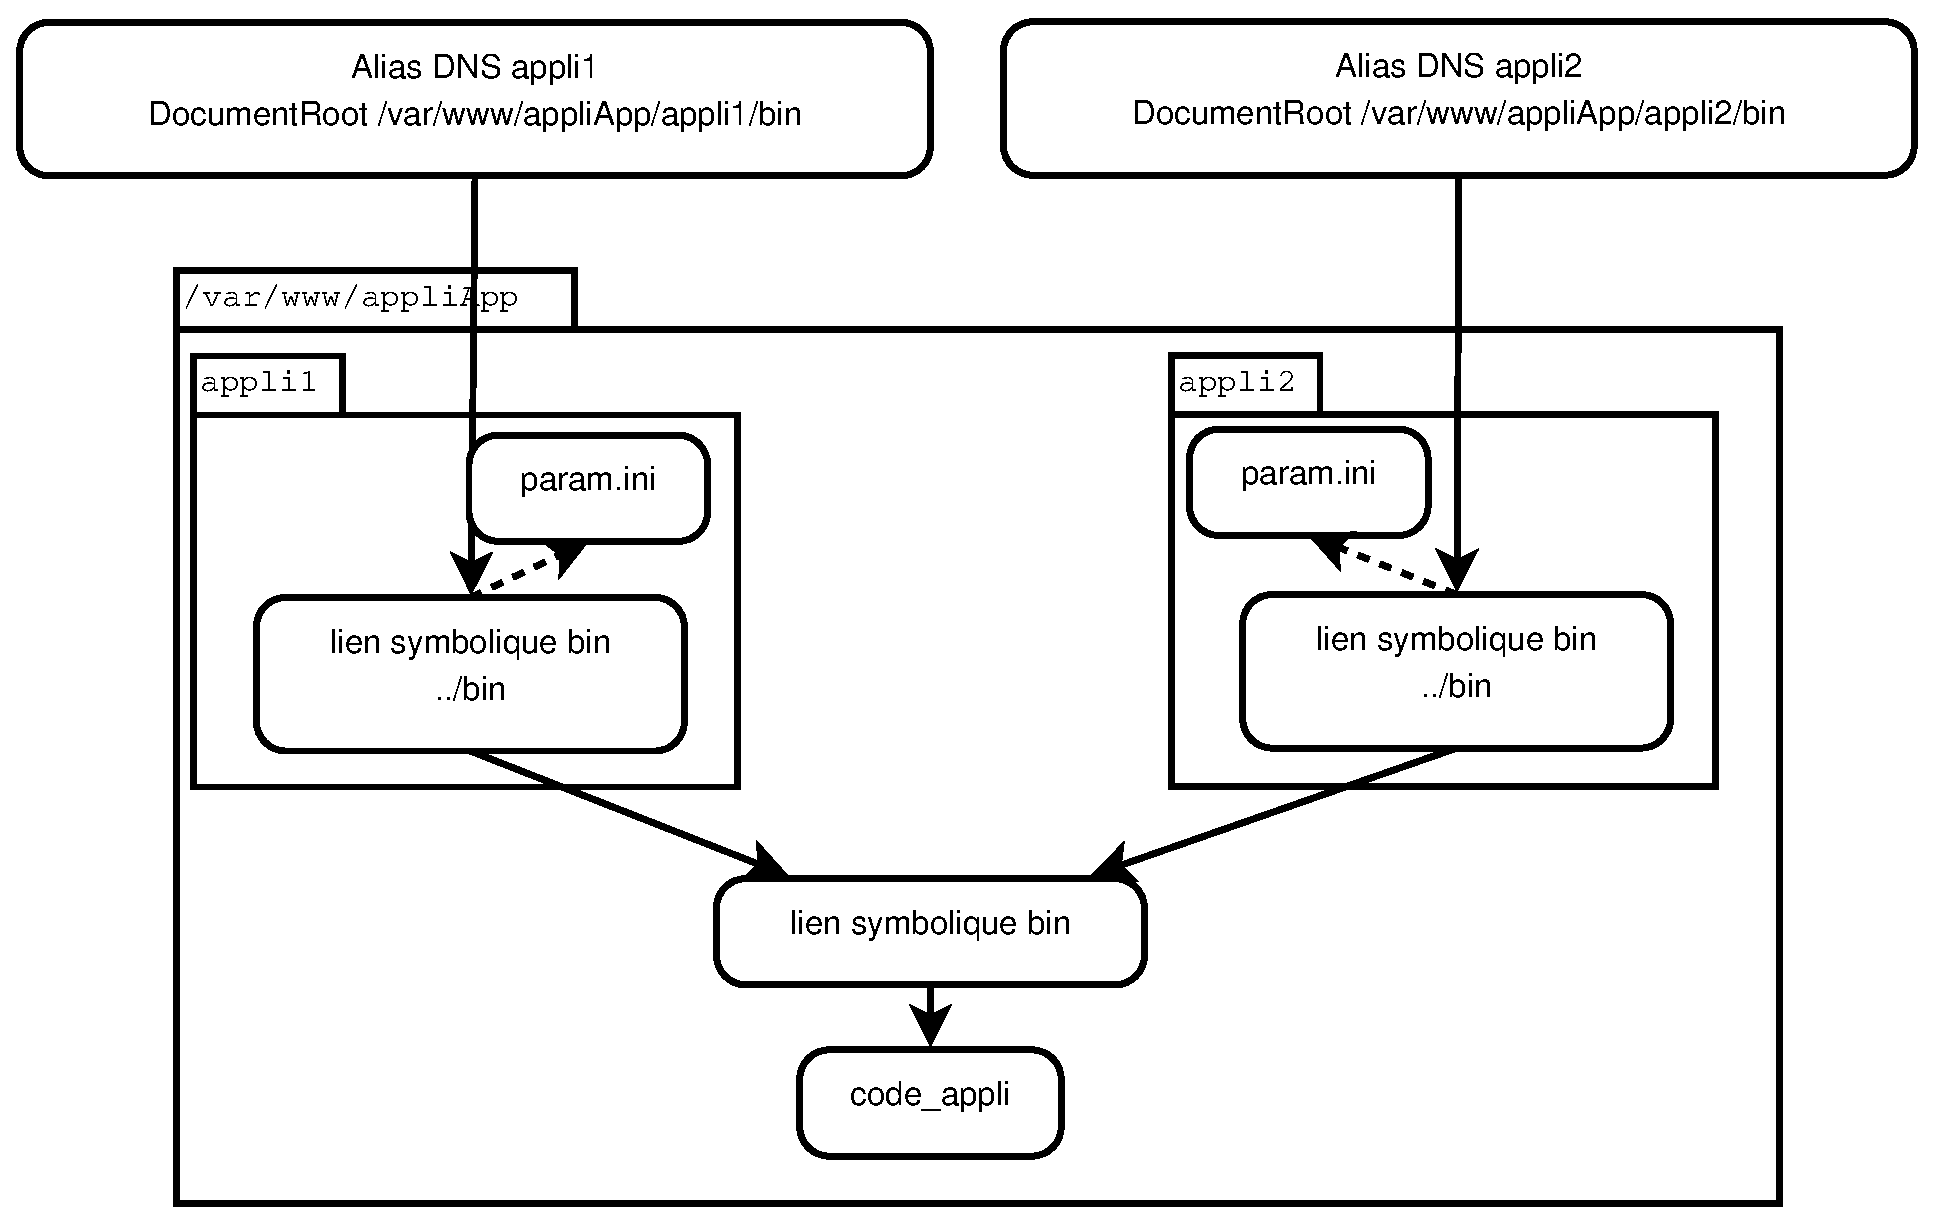
\includegraphics[width=\linewidth]{images/dnsmultiple}
\caption{\label{dnsmultipleschema}Schéma général d’implémentation pour utiliser le même code avec des noms d’application et des jeux de données différents}
\end{figure}

Dans le paramétrage de l’alias DNS (en principe, dans \textit{/etc/apache2/sites-available}), l’application pointe vers le dossier \textit{/var/www/appliApp/appli1/bin}. \textit{/var/www} correspond à la racine du site web, \textit{appliApp} au dossier racine de l’application, \textit{appli1} au dossier spécifique de l’alias DNS. Ce dossier \textit{appli1} ne contient que deux fichiers : \textit{param.ini}, qui contient les paramètres spécifiques, et \textit{bin}, qui est un lien symbolique vers le dossier \textit{../bin}.

Le dossier \textit{../bin} (donc, dans\textit{ /var/www/appliApp}) est lui aussi un alias qui pointe vers le code réel de l’application, ici \textit{code\_appli}. Le fichier \textit{param.inc.php} doit contenir les commandes suivantes pour que le fichier \textit{param.ini} soit correctement chargé selon le contexte :
\begin{lstlisting}
$chemin = substr($_SERVER["DOCUMENT_ROOT"],0, strpos($_SERVER["DOCUMENT_ROOT"],"/bin"));
$paramIniFile = "$chemin/param.ini";
\end{lstlisting}

Le fichier \textit{param.ini} sera cherché dans le dossier parent du code de l’application, c’est à dire soit dans \textit{appli1}, soit dans \textit{appli2} dans cet exemple. Il suffit qu’il contienne les paramètres adéquats pour rendre l’application utilisable dans des contextes différents à partir du même code initial.

Le fichier \textit{param.ini} est le dernier qui est traité par l'application pour récupérer les paramètres. Ceux-ci sont lus dans l'ordre suivant :

\textbf{param/param.default.inc.php $\rightarrow$ param/param.inc.php $\rightarrow$ ../param.ini}

\textit{param.ini} contiendra les entrées spécifiques liées au DNS utilisé pour accéder à l'application, en principe tout ou partie de celles-ci :
\begin{lstlisting}
BDD_schema=filo-science, public, gacl
BDD_login=compte_de_connexion
BDD_passwd=mot_de_passe_de_connexion
BDD_dsn=pgsql:host=serveur;dbname=base_de_donnees;sslmode=require
GACL_aco=filo
\end{lstlisting}

Si un libellé contient une apostrophe, la chaîne doit être insérée dans des guillemets doubles, comme ici pour la variable \textit{APPLI\_titre}.


\subsection{Droits à attribuer au serveur web}
\label{droitsApache}
Le serveur web doit pouvoir accéder en lecture à l'ensemble des fichiers de l'application, et en écriture à deux dossiers :
\begin{itemize}
\item \textit{display/templates\_c} : fichier utilisé par Smarty pour compiler les modèles de documents HTML ;
\item \textit{img} : dossier de génération des images et des fichiers temporaires.
\end{itemize}

Deux scripts sont fournis pour attribuer les droits : 
\begin{itemize}
\item \textbf{install/apache2/upgrade\_rights.sh} : positionne les droits en utilisant les droits standards Linux (owner, group)
\item \textbf{install/apache2/upgrade\_rights\_with\_acl.sh} : positionne les droits à partir des ACL.
\end{itemize}

Les scripts doivent être lancés ainsi :
\begin{lstlisting}
filo-2.0/install/apache2/upgrade_rights.sh v2.0
\end{lstlisting}
ou 
\begin{lstlisting}
filo-2.0/install/apache2/upgrade_rights_with_acl.sh v2.0
\end{lstlisting}


\section{Configurer l'application}

L'application est configurable par l'intermédiaire de trois fichiers :

\textbf{param/param.default.inc.php $\rightarrow$ param/param.inc.php $\rightarrow$ ../param.ini}

Le premier fichier contient les paramètres par défaut. Il est systématiquement fourni à chaque nouvelle version de l'application.

Le second est spécifique de l'implémentation. Il comprend notamment les informations liées à la connexion à la base de données, à la méthode d'identification, ou à la recherche des attributs dans l'annuaire LDAP. 

le troisième est destiné à offrir la possibilité d'accéder, à partir du même code applicatif, à plusieurs bases de données différentes (\textit{cf.} \ref{dnsmultiple} \textit{\nameref{dnsmultiple}}, page \pageref{dnsmultiple}).

Voici les principaux paramètres utilisés :

\subsection{Connexion à la base de données}

Dans la pratique, deux connexions sont nécessaires : l'une pour accéder à la base des droits, l'autre aux données proprement dites. Voici les paramètres à définir :

\begin{longtable}{|p{4cm}|p{11cm}|}
\hline
\textbf{Variable} & \textbf{Signification} \\
\hline
\endhead
BDD\_login & compte de connexion à la base de données \\
\hline
BDD\_passwd & mot de passe associé\\
\hline
BDD\_dsn & adresse de la base de données sous forme normalisée\\
\hline
BDD\_schema & schéma utilisé (plusieurs schémas peuvent être décrits, en les séparant par une virgule - fonctionnement propre à Postgresql)\\
\hline
GACL\_dblogin & compte de connexion à la base de données des droits\\
\hline
GACL\_dbpasswd & mot de passe associé\\
\hline
GACL\_dsn & adresse normalisée \\
\hline
GACL\_schema & schéma utilisé\\
\hline
GACL\_aco & nom du code de l'application utilisé dans la gestion des droits\\
\hline
\caption{Variables utilisées pour paramétrer les connexions}
\end{longtable}

\subsection{Identification des utilisateurs}

\begin{longtable}{|p{6cm}|p{10cm}|}
\hline
\textbf{Variable} & \textbf{Signification} \\
\hline
\endhead
ident\_type & Type d'identification supporté. L'application peut gérer \textbf{BDD} (uniquement en base de données),\textbf{LDAP} (uniquement à partir d'un annuaire LDAP) \textbf{LDAP-BDD} (d'abord identification en annuaire LDAP, puis en base de données), \textbf{CAS} (serveur d'identification \textit{Common Access Service}\footnote{serveur externe gérant l'identification des utilisateurs, et renvoyant à l'application le login utilisé}), et enfin \textbf{HEADER} (identification derrière un proxy qui fournit le login dans une variable d'entête HTTP)\\
\hline
CAS\_plugin & Nom du plugin utilisé pour une connexion CAS \\
\hline
CAS\_address & Adresse du serveur CAS\\
\hline
CAS\_port & Systématiquement 443 (connexion chiffrée)\\
\hline
CAS\_CApath & chemin d'accès au certificat du serveur CAS \\
\hline
LDAP & tableau contenant tous les paramètres nécessaires pour une identification LDAP \\
\hline
ident\_header\_login\_var & par défaut, AUTH\_USER. Nom de la variable qui contiendra le login dans le cas d'une identification en mode HEADER (le radical HTTP\_  ne doit pas être indiqué) \\
\hline
privateKey & clé privée utilisée pour générer les jetons d'identification (ré-identification automatique après une première connexion) \\
\hline
pubKey & clé publique utilisée pour générer les jetons d'identification \\
\hline
tokenIdentityValidity & durée de validité, en secondes, des jetons d'identification\\
\hline
MAIL\_enabled & Si à 1, l'envoi de mail est géré par l'application \\
\hline
CONNEXION\_max\_attemps & nombre maximum d'essais de connexion avant blocage temporaire du compte \\
\hline
CONNEXION\_blocking\_duration & durée de blocage du compte \\
\hline
APPLI\_mailToAdminPeriod & intervalle de temps entre l'envoi d'un mail de notification de blocage de compte à un administrateur \\
\hline
APPLI\_admin\_ttl & durée de vie d'une session d'administration (temps maximum entre deux accès à une page d'administration avant réidentification) \\
\hline
APPLI\_lostPassword & Si à 1, autorise la récupération du mot de passe perdu, par envoi d'un mail avec un lien chiffré. Nécessite également que MAIL\_enabled soit positionné à 1 \\
\hline

\caption{Variables utilisées pour paramétrer l'identification}
\end{longtable}

\subsubsection{Ré-identification par jeton}

L'application permet de conserver l'identification plus longtemps que celle définie dans le serveur, en rejouant la connexion avec un jeton d'identification chiffré. Cela évite, par exemple, de devoir se ré-identifier toutes les heures si on accède au logiciel à partir d'un terminal mobile (smartphone ou tablette, par exemple).

Les trois dernières variables permettent de configurer ce mode d'identification. 

Le framework peut générer un jeton chiffré après la première identification, qui sera analysé pour savoir si l'utilisateur peut être ré-identifié automatiquement.

Pour que ce mécanisme fonctionne, il faut :
\begin{itemize}
\item que le paramètre \textit{tokenIdentityValidity} ait une durée de validité supérieure à la durée de vie de la session. Il est raisonnable de ne pas fixer une durée de vie supérieure à une journée de travail (10 heures). Le cookie transmis est protégé ;
\item que les clés privée et publique, utilisées pour le chiffrement du jeton, soient accessibles au serveur web (variables \textit{privateKey} et \textit{publicKey}).
\end{itemize}

Les clés sont générées automatiquement avec le script d'installation automatique du serveur et de l'application.

Le jeton est chiffré avec la clé privée, ce qui lui permet d'être lu, le cas échéant, par l'application. Il contient le login et la date d'expiration. 

Si l'utilisateur déclenche une déconnexion, le jeton est supprimé.

Pour plus d'informations, consultez comment fonctionne le mécanisme de ré-identification par jeton \cite{token}.

\subsubsection{Identification par HEADER}

Dans ce mode d'identification, le serveur web est placé derrière un serveur d'identification, appelé proxy d'identification. L'adresse de l'application pointe vers ce dernier. 

Le proxy gère la connexion de l'utilisateur, et fournit à l'application le login dans une variable configurable. Cette variable est accessible dans le tableau \$\_SERVER, par exemple \$\_SERVER [ "HTTP\_AUTH\_USER" ].

Pour activer ce mécanisme, il faut modifier les paramètres suivants dans le fichier \textit{param.ini.php} :
\begin{lstlisting}
$ident_type = "HEADER";
$ident_header_login_var = "AUTH_USER";
\end{lstlisting}

la variable ne doit pas contenir la racine HTTP\_ (une fonction l'extrait automatiquement).

\subsection{Configuration de l'accès à l'annuaire LDAP}

Les paramètres LDAP sont stockés dans un tableau :
\begin{lstlisting}
$LDAP = array(
		"address"=>"localhost",
		"port" => 389,
		"rdn" => "cn=manager,dc=example,dc=com",
		"basedn" => "ou=people,ou=example,o=societe,c=fr",
		"user_attrib" => "uid",
		"v3" => true,
		"tls" => false,
		"groupSupport"=>true,
		"groupAttrib"=>"supannentiteaffectation",
		"commonNameAttrib"=>"displayname",
		"mailAttrib"=>"mail",
		'attributgroupname' => "cn",
		'attributloginname' => "memberuid",
		'basedngroup' => 'ou=example,o=societe,c=fr'
);
\end{lstlisting}


L'application peut non seulement identifier les utilisateurs auprès de l'annuaire LDAP, mais également récupérer les groupes auxquels ils appartiennent dans celui-ci.

Voici les paramètres à indiquer dans ce cas de figure (valable en principe pour tout annuaire compatible OpenLdap) : 
\begin{longtable}{|p{4cm}|p{11cm}|}
\hline
\textbf{Variable} & \textbf{Signification} \\
\hline
\endhead
address &  adresse de l'annuaire\\
\hline
port & 389 en mode non chiffré, 636 en mode chiffré\\
\hline
rdn & compte de connexion, si nécessaire \\
\hline
basedn & base de recherche des utilisateurs\\
\hline
user\_attrib & nom du champ contenant le login à tester\\
\hline
v3 & toujours à \textit{true}\\
\hline
tls & \textit{true} en mode chiffré\\
\hline
groupSupport & \textbf{true} si l'application recherche les groupes d'appartenance du login dans l'annuaire\\
\hline
groupAttrib & Nom de l'attribut contenant la liste des groupes d'appartenance\\
\hline
commonNameAttrib & Nom de l'attribut contenant le nom de l'utilisateur\\
\hline
mailAttrib & Nom de l'attribut contenant l'adresse mail de l'utilisateur\\
\hline
attributgroupname & Attribut contenant le nom du groupe lors de la recherche des groupes (cn par défaut)\\
\hline
attributloginname & attribut contenant les membres d'un groupe\\
\hline
basedngroup & base de recherche des groupes \\
\hline
\caption{Variables utilisées pour paramétrer l'accès à l'annuaire LDAP}
\end{longtable}

\subsection{Paramètres spécifiques}
\label{paramspec}

\begin{longtable}{|p{4cm}|p{11cm}|}
\hline
\textbf{Variable} & \textbf{Signification} \\
\hline
\endhead
APPLI\_photoStockage & dossier contenant les photos générées par l'application, avant transmission au navigateur. Par défaut : \textit{img}\\
\hline
APPLI\_maxfilesize & Taille maximale des photos téléchargeables. Par défaut : 100000000 \\
\hline

\caption{Variables spécifiques}
\end{longtable}

\subsection{Paramètres stockés en base de données}
\label{paramdb}

À partir de la version 2, certains paramètres peuvent être stockés dans la base de données, pour éviter qu'ils ne soient dépendants de la configuration du serveur.

Ces paramètres sont accessibles depuis le menu \textit{administration}, item \textit{Paramètres de l'application}.

Voici la liste des paramètres actuellement décrits :
\begin{longtable}{|p{4cm}|p{11cm}|}
\hline
\textbf{Variable} & \textbf{Signification} \\
\hline
\endhead
APPLI\_title & Titre de l'application tel qu'il figure entre l'icône et le menu\\
\hline
mapDefaultLat & Latitude de positionnement par défaut des cartes \\
\hline
mapDefaultLong & Longitude de positionnement par défaut des cartes \\
\hline
mapDefaultZoom & Niveau de zoom des cartes par défaut \\
\hline
\caption{Paramètres stockés dans la base de données}
\end{longtable}


\section{Créer la base de données}

La base de données est composée de deux schémas : l'un pour stocker les informations d'identification, les droits d'accès et les traces (gacl), l'autre pour les données proprement dites (filo).

Le schéma \textit{public} ne devrait jamais être utilisé pour stocker l'information : réservez-le pour les composants communs, comme Postgis.

Les tables de gestion des droits peuvent être communes à plusieurs jeux / applications différentes : la variable \textit{GACL\_aco} permet de séparer la gestion des droits pour chaque application, tout en travaillant à partir des mêmes utilisateurs (répartis le cas échéant dans des groupes différents selon le jeu de données considéré).

Les tables sont créées à partir du script \textit{install/pgsql/create\_db.sql}.


Un compte d'administration par défaut est créé automatiquement :
\begin{itemize}
\item login : \textbf{admin}
\item mot de passe : \textbf{password}
\end{itemize}

Il devra être supprimé quand un autre compte d'administration aura été créé.


\subsection{Login de connexion}

Si la base de données et l'application sont hébergés dans deux serveurs différents, il est fortement conseillé de créer deux logins de connexion, un pour le schéma des droits, l'autre pour les schémas applicatifs. Ces logins ne doivent pouvoir être utilisés que depuis le serveur web hébergeant l'application.

Cette opération est possible en modifiant le fichier \textit{/etc/postgresql/9.5/main/pg\_hba.conf} selon ce principe :

\begin{lstlisting}
# Connexions pour les serveurs web 
host nom_database userGacl adresse_serveur/32 md5 
host nom_database userData adresse_serveur/32 md5
\end{lstlisting}

Le login utilisé dans \textit{userGacl} correspond à la variable \textit{\$GACL\_dblogin}, et \textit{userData} à \textit{\$BDD\_login}.

et en rechargeant ensuite la configuration de Postgresql avec la commande :
\begin{lstlisting}
service postgresql reload
\end{lstlisting}

\subsection{Droits sur les tables}

Le compte utilisé pour la connexion au schéma des droits doit pouvoir modifier les informations présentes dans l'ensemble des tables de \textit{gacl}. Il ne devrait pas pouvoir accéder aux autres schémas (hormis \textit{public}), sauf en cas d'installation mono-serveur (base de données hébergée dans la même machine et connexion à distance impossible).

Le compte utilisé pour accéder aux schémas des données doit pouvoir modifier l'ensemble des informations dans les schémas de données, et lire la table \textit{gacl.aclgroup}.

Le plus simple est d'utiliser le logiciel \textit{pgAdmin} \cite{pgadmin} pour attribuer les droits.

Le script d'installation automatique rend le compte \textit{filo} propriétaire de la base de données, ce qui simplifie la gestion des droits sur les tables.

\subsection{Scripts de modification}

Lors de la livraison de nouvelles versions, il est possible que des scripts de modification soient livrés pour mettre à niveau la base de données. Ces scripts doivent être exécutés dans tous les schémas contenant des données applicatives (pour plus de détails, consultez ci-après \textit{\nameref{newVersion}}).

\section{Mise en production}

Une fois l'application configurée, et après avoir créé un nouveau compte d'administration :
\begin{itemize}
\item supprimez le compte \textit{admin}, livré par défaut, qui ne doit pas être conservé. Sa désactivation n'est pas suffisante : si pour une raison ou pour une autre le compte est réactivé, n'importe qui pourra récupérer les droits totaux ;
\item supprimez le dossier \textit{install} qui contient les scripts de création des tables ;
\item déplacez le dossier \textit{database}, qui contient la documentation d'installation et de configuration (elle n'a pas à rester accessible depuis le site web) ;
\item faites une revue des droits, pour vous assurer que tout est correctement configuré.
\end{itemize}

Vous pouvez également tester si la configuration du serveur est correcte en recourant à \textit{ZAProxy} \cite{zaproxy}, qui analysera la communication entre le serveur et un navigateur et identifiera les problèmes éventuels de non conformité (mauvaise réécriture des entêtes HTML suite à une mauvaise configuration du serveur Apache, par exemple).

\section{Installer une nouvelle version}
\label{newVersion}

\subsection{Faites une sauvegarde de la base de données}
Il arrive fréquemment que la structure de la base de données évolue. Avant toute opération, assurez-vous de disposer d'une sauvegarde, dans un autre support.

Un programme de sauvegarde est disponible dans \textit{install/pgsql/backup.sh}. Vous pouvez l'exécuter manuellement ainsi :
\begin{lstlisting}
su postgres -c "install/pgsql/backup.sh"
\end{lstlisting}

La sauvegarde sera stockée dans \textbf{/var/lib/postgresql/backup}.

Si vous avez utilisé le script d'installation automatique, le programme est également présent dans \textit{/var/lib/postgresql}.

\subsection{Procédure automatique de mise à jour}

Si l'application est installée dans un serveur dédié à cet usage (installation réalisée avec le script \href{https://github.com/Irstea/filo-science/blob/master/install/deploy_new_instance.sh}{https://github.com/Irstea/filo-science/blob/master/install/deploy\_new\_instance.sh}), un script de mise à jour automatique peut être téléchargé. Il est disponible dans le dossier\\ \href{https://github.com/Irstea/filo-science/tree/master/install}{https://github.com/Irstea/filo-science/tree/master/install}, et est sous la forme :
\begin{lstlisting}
upgrade-2.0-2.1.sh
\end{lstlisting}
où \textbf{2.0} correspond à la version courante de votre installation, et \textbf{2.1} à la version cible.

Pour utiliser ce script :
\begin{lstlisting}
sudo -s
wget https://github.com/Irstea/filo-science/raw/master/install/upgrade-2.0-2.1.sh
chmod +x upgrade-2.0-2.1.sh
./upgrade-2.0-2.1.sh
\end{lstlisting}

Le script va télécharger le code de la nouvelle version et mettra à jour la base de données, si c'est nécessaire.

\subsection{Sauvegarder le fichier contenant les paramètres de l'application}

Le fichier \textit{param/param.inc.php} contient vos paramétrages spécifiques. Lors de l'installation d'une nouvelle version, il va être supprimé.

Faites-en une copie, et remettez-le en place après avoir installé la nouvelle version.

\subsection{Consultez le fichier news.txt}

Le fichier \textit{param/news.txt} contient la description des modifications apportées au logiciel. Il précise notamment si une mise à jour de la base de données doit être appliquée.

\subsection{Mise à jour de la structure de la base de données}

Le dossier \textit{install/pgsql} contient les scripts de création et de mise à jour de la base de données. Les scripts de mise à jour sont nommés ainsi :
\begin{lstlisting}
alter_versionAnterieure-versionMiseAJour.sql
\end{lstlisting}

\textit{versionAnterieure} correspond à la version la plus ancienne qui doit être mise à jour, \textit{versionMiseAJour} la version cible. Par exemple :
\begin{lstlisting}
alter_2.0-2.1.sql
\end{lstlisting}
indique que toutes les versions entre \textit{2.0} et \textit{2.1} doivent être mises à jour avec le script indiqué. Si vous avez \og sauté \fg{} certaines versions du logiciel, il est possible que plusieurs scripts doivent être appliqués.

La mise à jour doit être appliquée dans tous les schémas contenant des données, notamment dans le cas où le même logiciel est utilisé pour gérer plusieurs jeux de données.

Avant d'exécuter les scripts, vérifiez leur contenu, et notamment le nom des schémas.

Ne relancez jamais l'exécution d'un script.

\subsection{Reconfigurer les droits d'accès au serveur web}

Après installation de la nouvelle version du code, n'oubliez-pas de reconfigurer les accès en lecture pour le compte utilisé pour faire fonctionner le serveur web, et en écriture pour les dossiers \textit{img} et \textit{display/templates\_c} (\textit{cf.} \ref{droitsApache} \textit{\nameref{droitsApache}}, page \pageref{droitsApache}).

\subsection{Supprimer les dossiers inutiles}
Une fois la mise en production validée, supprimez le dossier \textit{install} et déplacez le dossier \textit{database}, et faites une revue des droits pour vous assurer qu'il n'y a pas eu de modification intempestive ou que la configuration est toujours correcte.

\subsection{Vérifier la configuration du chiffrement}
Avec un navigateur récent, ou en testant le site (s'il est accessible depuis internet) à partir de \href{https://www.ssllabs.com/ssltest/}{SSLLABS}, vérifiez que l'application soit correctement configurée, notamment au niveau du serveur Apache.

\chapter{Administrer l'application}

\section{Gérer les droits}
\label{droits}


\subsection{Principe général}

Les droits sont gérés selon le principe initialement utilisé dans la bibliothèque PHPGACL \cite{phpgacl}, aujourd'hui obsolète. 

Les logins sont déclarés dans des groupes organisés de manière hiérarchique : un groupe hérite des droits attribués à ses parents.

Les droits utilisés dans le logiciel sont associés à des groupes. Il est possible d'attribuer plusieurs droits à un même groupe, et un droit peut être détenu par des groupes différents.

Si le paramètre \textit{\$LDAP["groupSupport"]} est positionné à \textit{true}, les groupes dont fait partie le compte LDAP sont également récupérés. Si ces groupes se voient attribués des droits, les comptes associés les récupéreront automatiquement.

Voici le schéma des tables utilisées pour gérer les droits :

\begin{figure}[H]
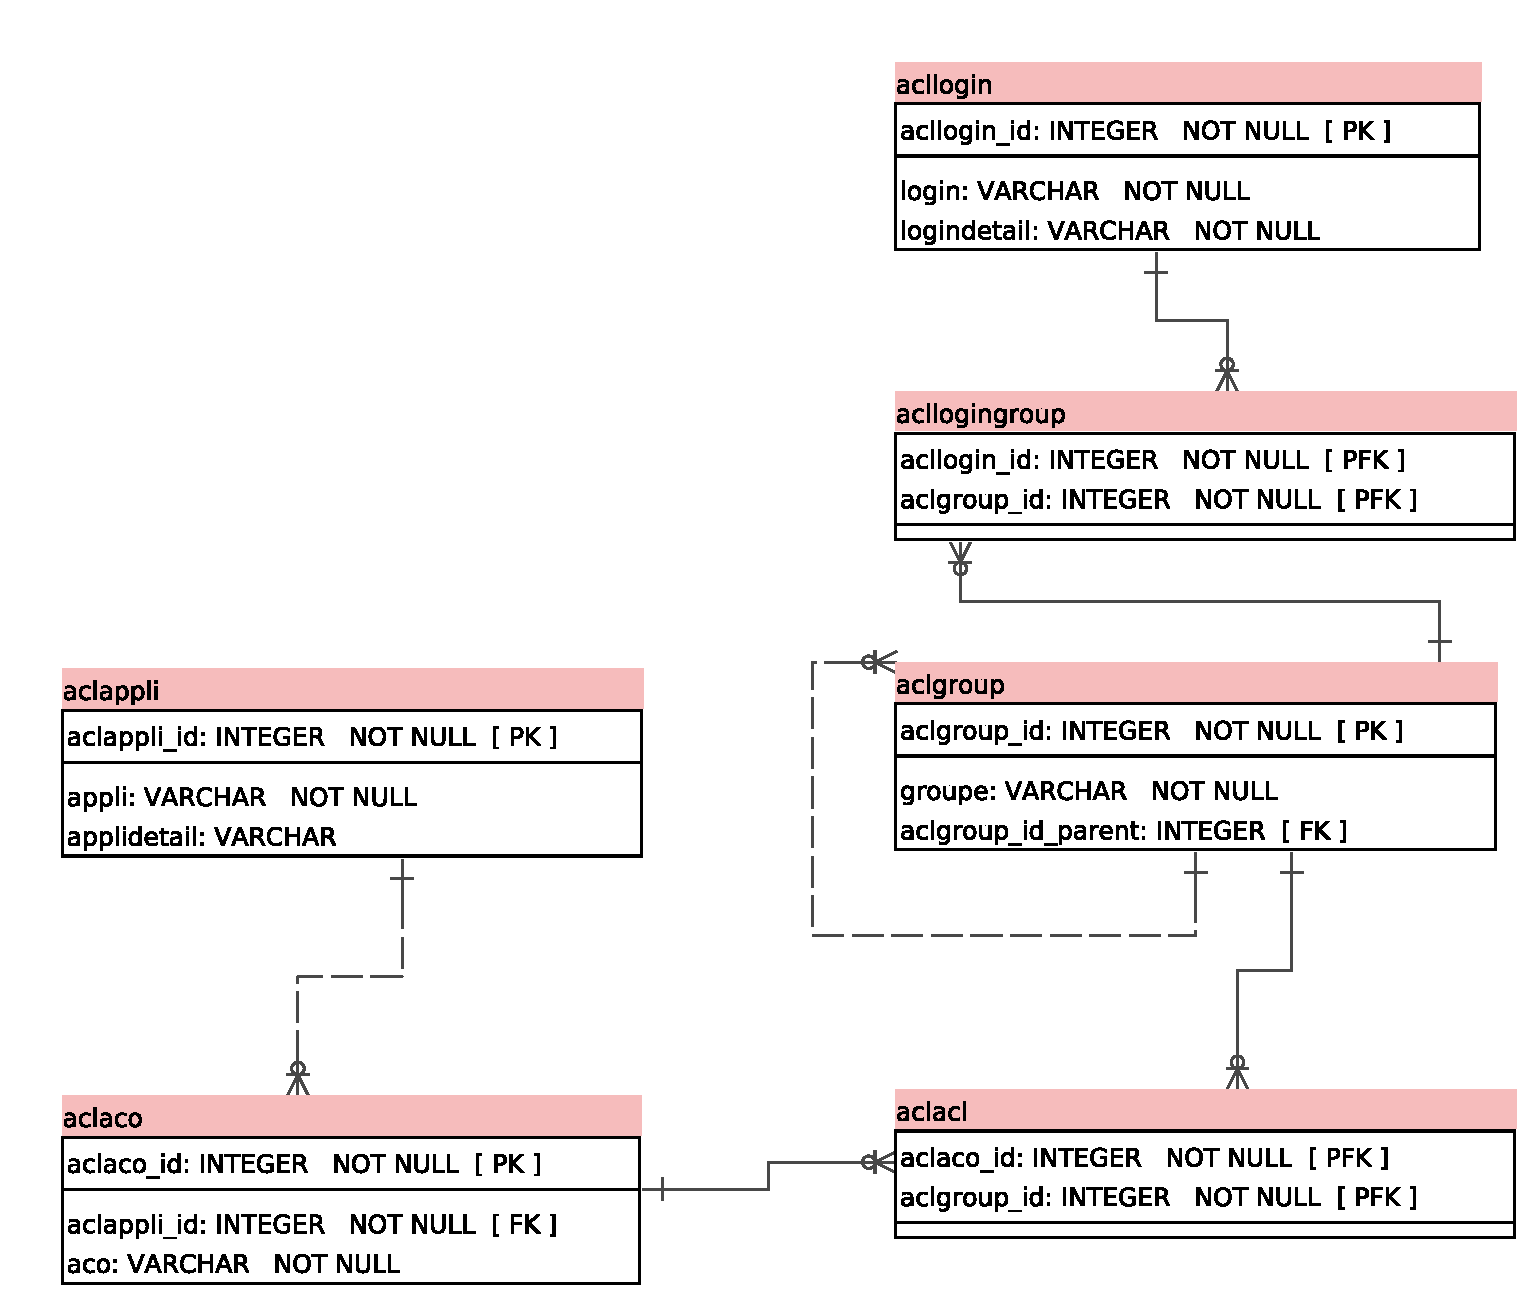
\includegraphics[width=\linewidth]{images/acl_only}
\caption{Schéma des tables utilisées pour gérer les droits}
\end{figure}

Voici la description des tables :
\begin{description}
\item[acllogin] : liste des logins utilisés. Si un compte est créé dans la base locale d'identification, un enregistrement est également créé dans cette table. Pour les identifications LDAP ou CAS, ils doivent être identiques. Si seuls les groupes LDAP sont utilisés pour un compte, il n'a pas besoin d'être décrit ici ;
\item[aclappli] : liste des applications gérées. Il est possible de gérer, à partir de la même base de données, plusieurs ensembles de droits, qui utilisent les mêmes logins.
\item[aclaco] : liste des droits déclarés dans l'application ;
\item[aclgroup] : liste des groupes contenant les logins, et qui détiennent les droits. Un groupe peut hériter d'un autre groupe. Les droits associés au groupe parent sont également attribués au groupe hérité ;
\item[acllogingroup] : table permettant de déclarer les logins associés à un groupe ;
\item[aclacl] : table décrivant les droits détenus par un groupe.
\end{description}

Le module d'administration permet de saisir toutes ces informations. Il faut que l'utilisateur dispose du droit \textit{admin}, c'est à dire qu'il fasse partie du groupe \textit{admin} (configuration par défaut à l'initialisation de la base des droits) pour pouvoir accéder à ces fonctions.

\subsection{Créer un nouvel utilisateur}

Les utilisateurs peuvent être issus soit de l'annuaire LDAP, soit de la base interne. 
Pour créer un nouvel utilisateur dans la base locale :
\begin{itemize}
\item \textit{Administration $\rightarrow$ Liste des comptes }
\item \textit{Nouveau login}
\item renseignez au minimum le login.
\end{itemize}

\begin{figure}[H]
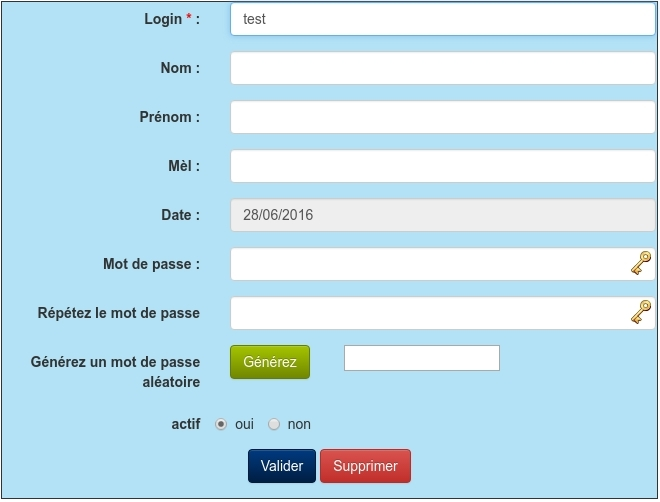
\includegraphics[width=\linewidth]{images/user_create}
\caption{Écran de saisie d'un login de connexion}
\end{figure}

Pour créer le mot de passe, vous pouvez cliquer sur le bouton \textit{Générez}, qui  en générera un automatiquement. Envoyez-le par mél à son destinataire (par \textit{copier-coller}), en lui demandant de le modifier à la première connexion (icône en forme de clé, dans le bandeau, en haut à droite).

Les mots de passe doivent respecter les règles suivantes :
\begin{itemize}
\item ils doivent avoir une longueur minimale de 10 caractères ;
\item ils doivent comprendre trois types de caractères différents parmi les minuscules, majuscules, chiffres et caractères de ponctuation ;
\item ils ne peuvent pas être réutilisés pour le même login ;
\item les mots de passe n'expirent pas.
\end{itemize}

Les mots de passe sont stockés sous forme d'empreinte, calculée en rajoutant un sel\footnote{chaîne de caractère rajoutée au mot de passe -- en général le login ou un identifiant -- qui permet d'éviter que deux mots de passe identiques, associés à deux logins différents, aient la même empreinte} et encodés en SHA256 : ils ne peuvent pas être retrouvés en cas de perte.

L'application n'intègre pas de module permettant de régénérer automatiquement un mot de passe en cas de perte : c'est au responsable applicatif d'en fournir un nouveau.

La création d'un compte entraîne la création d'une entrée identique dans la table des \textit{acllogin}, utilisée pour attribuer les droits.

Pour désactiver temporairement un compte, sélectionnez \textit{non} dans la zone \textit{actif}. Si le compte ne doit plus être utilisé, supprimez-le.

Attention : si le compte disposait des droits d'administration, assurez-vous que vous avez toujours un compte disposant des mêmes droits avant la suppression.

\subsection{Créer un login utilisé dans la gestion des droits}

Indépendamment du compte de connexion, qui peut être soit issu de la base interne, soit récupéré auprès d'un annuaire LDAP ou d'un serveur CAS, l'application a besoin de connaître les utilisateurs pour pouvoir leur attribuer des droits.

À partir du menu, choisissez \textit{Administration $\rightarrow$ ACL - logins}.

Vous pouvez modifier un login existant ou en créer un nouveau. Dans ce cas, vous devrez indiquer au minimum le login utilisé (identique à celui qui est employé pour la connexion à l'application : base de données interne, annuaire LDAP, serveur CAS).

\begin{figure}[H]
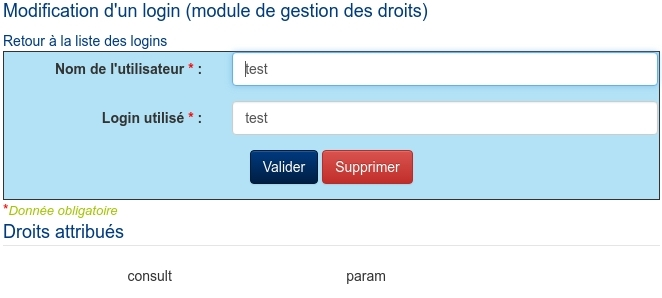
\includegraphics[width=\linewidth]{images/acl_login}
\caption{Écran de modification d'un login dans le module de gestion des droits}
\end{figure}


Sous l'écran de saisie figurent la liste des droits attribués à un login (en modification, le calcul n'est réalisé qu'à l'affichage de la page).

\subsection{Définir les groupes d'utilisateur}

Les groupes d'utilisateurs sont gérés selon un mécanisme d'héritage. Un groupe de haut niveau hérite des groupes précédents : si des droits ont été attribués à un groupe de niveau inférieur, un login associé à un groupe de niveau supérieur les récupère également.

Pour définir les groupes, dans le menu, choisissez \textit{Administration $\rightarrow$ ACL - groupes de logins}.

\begin{figure}[H]
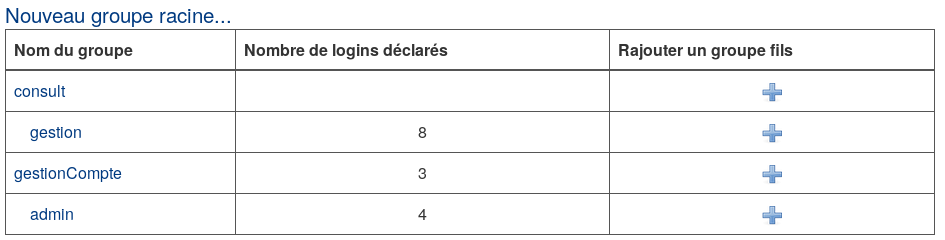
\includegraphics[width=\linewidth]{images/acl_groupe.png}
\caption{Liste des groupes de logins}
\end{figure}

Ainsi, le login déclaré dans le groupe \textit{admin} récupérera les droits attribués aux groupes \textit{gestionCompte}.

Pour créer un groupe, il existe deux possibilités :
\begin{itemize}
\item soit le groupe est à la base d'une nouvelle branche : utilisez alors \textit{Nouveau groupe racine...} ;
\item soit le groupe hérite d'un autre groupe : cliquez sur le signe + (\textit{Rajouter un groupe fils}).
\end{itemize}

Vous pouvez indiquer les logins qui sont rattachés à ce groupe.


\subsection{Créer une application}
Le moteur utilisé pour faire fonctionner le logiciel Otolithe permet de gérer des droits différents pour des jeux de données différents, à partir du même code applicatif. Chaque couple \textit{logiciel} $\leftrightarrow$ \textit{base de données} constitue donc une \textit{application}, au sens de la gestion des droits.

Il est ainsi possible, à partir de la même base de données, de définir des droits différents selon les jeux de données utilisés (un jeu de données correspond à un schéma de base de données comprenant l'intégralité des tables applicatives).

À partir du menu, choisissez \textit{Administration $\rightarrow$ ACL - droits} :

\begin{figure}[H]
\centering
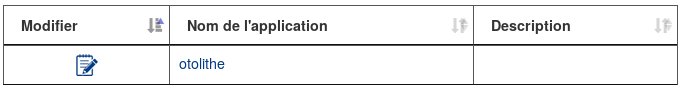
\includegraphics[width=0.7\linewidth]{images/liste_appli.png}
\caption{Liste des applications déclarées}
\end{figure}

Pour créer une nouvelle application, choisissez \textit{Nouvelle application...}. 

\begin{figure}[H]
\centering
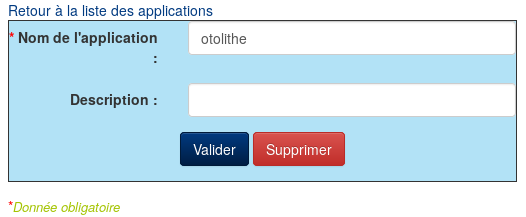
\includegraphics[width=0.7\linewidth]{images/appli_change.png}
\caption{Écran de saisie d'une application}
\end{figure}

Le nom de l'application doit impérativement correspondre à la valeur \textit{\$GACL\_appli} dans les fichiers de paramètres : c'est ce qui permet au framework de savoir quels droits appliquer.

\subsection{Définir les droits utilisables dans l'application}

À partir de la liste des applications, cliquez sur le nom de celle pour laquelle vous voulez définir les droits utilisables. 
À partir de la liste, sélectionnez \textit{Nouveau droit...}.

\begin{figure}[H]
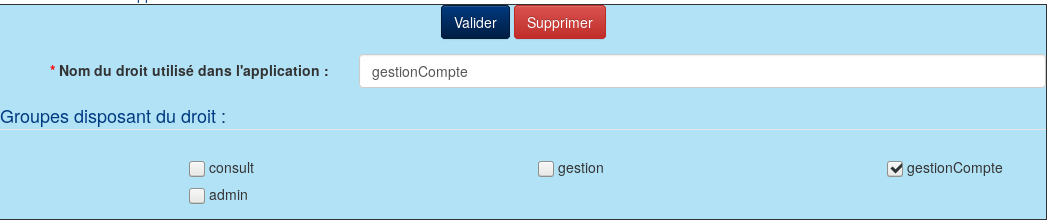
\includegraphics[width=\linewidth]{images/appli_droit.png}
\caption{Écran de saisie des droits associés à une application}
\label{applidroit}
\end{figure}

Le nom du droit doit être celui défini dans le corps de l'application (les droits sont positionnés dans les fichiers \textit{param/actions.xml}, qui contient la liste des modules utilisables, et \textit{param/menu.xml}, qui sert à générer le menu -- \textit{cf.} table \ref{droitsCollec} \textit{\nameref{droitsCollec}}, page \pageref{droitsCollec}).

Indiquez les groupes d'utilisateurs qui seront associés au droit courant.

\subsection{Cas particulier des groupes et des logins issus d'un annuaire LDAP}

Si vous avez paramétré l'application pour qu'elle s'appuie sur un annuaire LDAP pour gérer l'affectation des utilisateurs dans les groupes, vous n'êtes pas obligés de les déclarer explicitement dans le module de gestion des droits.

\subsubsection{Droits attribués à un groupe LDAP}

Tous les utilisateurs d'un groupe héritent d'un droit dans l'application.

\begin{itemize}
\item définissez le nom du groupe (en respectant la casse) dans le tableau des groupes d'utilisateurs (par exemple, EABX) ;
\item sélectionnez le nom de ce groupe dans les droits utilisables ;
\item tous les utilisateurs de l'annuaire LDAP récupéreront automatiquement les droits attribués à ce groupe.
\end{itemize}

\subsubsection{Droits attribués à un utilisateur particulier de l'annuaire LDAP}

Un utilisateur s'identifie auprès de l'annuaire LDAP, mais dispose de droits particuliers.

\begin{itemize}
\item créez son login dans la gestion des droits ;
\item rajoutez-le dans le groupe d'utilisateurs adéquat.
\end{itemize}


\section{Droits spécifiques de l'application Filo-Science}

\subsection{Droits à positionner}
Voici les droits nécessaires pour faire fonctionner correctement l'application :

\begin{longtable}{|p{5cm}|p{10cm}|}
\hline
\textbf{Droit} & \textbf{Usage} \\
\hline
\endhead
admin &	Gestion des utilisateurs, des droits, des paramètres globaux de l'application\\
\hline
param &	Gestion des paramètres, création des projets, etc.\\
\hline
gestion &	Création d'un protocole, saisie des opérations de pêche, pour les projets rattachés au groupe de l'utilisateur \\
\hline
consult	& Droit technique, permettant la consultation des informations générales, sans possibilité de modification\\
\hline


\caption{\label{droitsCollec}Liste des droits utilisés}
\end{longtable}

Ces droits doivent être définis pour chaque application (couple \textit{logiciel} $\leftrightarrow$ \textit{base de données}) gérée par la base de gestion des droits.

\section{Gestion des traces}

Tous les appels lancés par les utilisateurs vers les modules de l'application sont enregistrés dans la table \textit{gacl.log}, qui ne doit être accessible qu'aux personnes dûment autorisées. Les traces sont supprimées au bout d'un an (script de nettoyage exécuté lors de la connexion d'un utilisateur).

Voici un exemple de trace générée :
\begin{lstlisting}
log_id	login	nom_module	log_date	commentaire	ipaddress
1	admin	filo-operationDisplay	2019-04-30 17:23:01	ok	127.0.0.1
2	admin	filo-projectList	2019-04-30 17:23:05	ok	127.0.0.1
3	admin	filo-projectChange	2019-04-30 17:23:07	ok	127.0.0.1
4	admin	filo-projectWrite	2019-04-30 17:23:15	ok	127.0.0.1
5	admin	filo-project-write	2019-04-30 17:23:15	1	127.0.0.1

\end{lstlisting}

La colonne \textit{commentaire} précise des informations concernant soit la connexion, soit l'écriture en base de données : dans ce cas, l'identifiant considéré est indiqué.
L'adresse IP est en principe celle de l'utilisateur, y compris en prenant en compte le passage par un serveur Reverse-proxy\footnote{serveur mis en entrée du réseau privé, qui permet de masquer les adresses internes et de contrôler les accès depuis Internet}.

Parallèlement, les messages d'erreur sont envoyés au processus Linux SYSLOG, qui enregistre les traces dans le fichier \textit{/var/log/apache2/error.log}.

\chapter{Importations et exportations de données}

\section{Présentation}

Le logiciel Filo-Science intègre deux modules génériques permettant de réaliser soit des importations, soit des exportations. 
Le premier vise à importer des données de pistage de poissons ou des données transmises par des sondes d'analyse physico-chimique. Les données fournies sont de type tabulé (fichiers ressemblant à des fichiers CSV).
Le second sert à générer un export de données au format JSON, pouvant comprendre également les informations rattachées, pour pouvoir les réimporter dans une autre base de données.

Les tables qui permettent de décrire ces fonctions sont stockées dans le schéma \textit{import} (figure \ref{fig:export_schema}).
\begin{figure}[h!]
\begin{center}
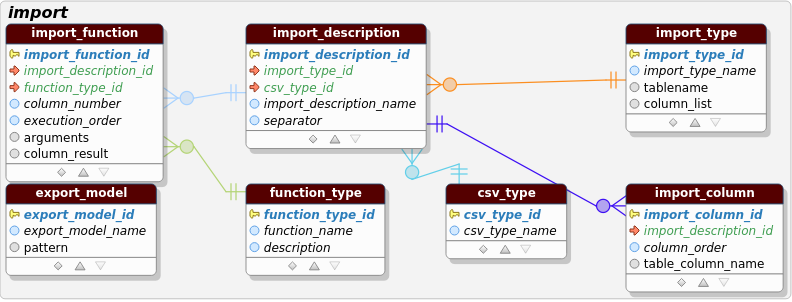
\includegraphics[width=\linewidth]{images/export_schema}
\captionof{figure}{Schéma des tables utilisées pour décrire les importations/exportations}
\label{fig:export_schema}
\end{center}
\end{figure}

\section{Importation de données tabulées}

Les structures des fichiers fournis par les systèmes d'acquisition automatique sont très variées, les données nécessitent souvent d'être reformatées ou recalculées avant de pouvoir être importées dans une table.

Le principe d'importation est le suivant :
\begin{itemize}
	\item chaque champ (une colonne) du fichier à importer peut faire l'objet d'une ou plusieurs transformations ou contrôles ;
	\item une fois l'ensemble de ces opérations réalisées, les champs pertinents vont être assignés à des colonnes de la table cible, et l'enregistrement réalisé en base de données.
\end{itemize}

\subsection{Types d'import}

Trois types d'import sont décrits et fournis, qui permettront d'alimenter les tables \textit{detection}, \textit{probe\_measure} et \textit{location}. 
La liste des colonnes utilisables pour l'importation est décrite, chaque colonne étant séparée par une virgule.

Les types d'import ne doivent pas être modifiés.

\subsection{Types de fonctions}

Les fonctions, codées dans l'application, sont décrites dans la table \textit{function\_type}. Cette table ne peut pas être modifiée.

La table \ref{tab:fonctions} présente la liste des fonctions utilisables pour préparer un import.

\begin{longtable}{|c|>{\raggedright\arraybackslash}p{5cm}|c|c|}
\caption{Liste des fonctions utilisées pour préparer un import.} \label{tab:fonctions} \\

\hline \multicolumn{1}{|c|}{\textbf{Nom de la fonction}} & \multicolumn{1}{c|}{\textbf{Description}} & \multicolumn{1}{c|}{\textbf{Contrôle ?}} & \multicolumn{1}{c|}{\textbf{Transformation ?}} \\ \hline 
\endfirsthead

\multicolumn{4}{c}%
{{\bfseries \tablename\ \thetable{} -- suite de la page précédente}} \\
\hline \multicolumn{1}{|c|}{\textbf{Nom de la fonction}} & \multicolumn{1}{c|}{\textbf{Description}} & \multicolumn{1}{c|}{\textbf{Contrôle ?}} & \multicolumn{1}{c|}{\textbf{Transformation ?}} \\ \hline 
\endhead

\hline \multicolumn{4}{|r|}{{Suite sur la page suivante}} \\ \hline
\endfoot

 \hline
\endlastfoot

testValue & Teste si un champ contient la valeur indiquée & X &  \\ 
getSecondsFromTime & Transforme un champ de type hh:mm:ss.u en ss.u &  & X \\ 
extractRightChar & Extrait les n caractères à droite du champ &  & X \\ 
concatenateDateAndTime & Concatène un champ date et un champ time. L'argument doit correspondre au numéro de la colonne time &  & X \\ 
transformJulianToDate & Transforme un nombre de jours depuis la date indiquée en référence (au format Y-m-d) en date exploitable au format Y-m-d &  & X \\ 
verifyTypeNumber & Vérifie si une valeur est numérique ou non & X &  \\ 
testColumnsNumber & Vérifie que le nombre de colonnes de la ligne courante correspond bien au nombre attendu &  & X \\ 
getIndividualFromTag & Récupère l'identifiant du poisson à partir du tag (RFID) &  & X \\ 
getIndividualFromTransmitter & Récupère l'identifiant du poisson à partir du transmetteur (radio ou acoustique) &  & X \\ 
numericToHexa & Transforme une valeur numérique en valeur Hexa, si celle-ci ne l'est pas. La valeur Hexa doit comprendre au moins une lettre.  &  & X \\ 
concatenate & Associe le contenu de colonnes ou du texte. L'argument doit être au format JSON, sous la forme : [{"type":"col","val":4}, {type:"str","val":":"}] &  &  \\ 
matchingCode & Remplace la valeur courante par une autre valeur, définie dans un argument JSON au format : {"valueSearched":correspondingValue, "2ndvalue":corresp2}. Pour la recherche des paramètres de sonde, valueSearched doit correspondre au libellé utilisé par la sonde, et correspondingValue à la valeur de la clé dans la table des paramètres &  & X \\ 
formatDateTime & Transforme une datetime dans un format reconnu par la base de données, à partir du format indiqué. Exemple : d/m/Y H:i:s pour une date de type 13/01/2019 08:50:00. La liste des formats autorisés est disponible ici : \href{https://www.php.net/manual/fr/datetime.createfromformat.php}{https://www.php.net/ manual/fr/datetime.createfromformat.php}&  & X \\ 
decodeAll & Transforme un jeu de caractère particulier en UTF-8. L'argument doit comprendre le jeu de caractère à transcoder, par exemple UTF-32. C'est l'ensemble de la ligne qui sera transcodé &  & X \\ 
transformDecimalSeparator & Transforme la virgule en point, pour les champs décimaux en français &  & X \\ 
\hline 

\end{longtable}

\subsection{Créer un modèle d'import}

Ouvrez le menu \textit{Télédétection > Paramètres > Modèles d'import}, puis cliquez sur le lien \textit{Nouveau modèle}. Les informations à renseigner sont les suivantes :
\begin{itemize}
	\item Type d'import : 
	\begin{itemize}
		\item Détection : données de détections enregistrées depuis une station fixe
		\item Données de sonde : relevés physico-chimiques réalisés par une sonde
		\item Détections manuelles : données de détection réalisées sur le terrain.
	\end{itemize}
	\item Type de fichier CSV :
	\begin{itemize}
		\item Data in columns : format classique des fichiers CSV. Une colonne contient toujours la même information
		\item Data in lines : chaque ligne décrit le paramètre relevé et la valeur associée
	\end{itemize}
	\item  Nom du modèle : nom mnémotechnique
	\item Séparateur de champs : indiquez le séparateur utilisé (point-virgule, virgule, tabulation, espace).
\end{itemize}

Une fois ces informations enregistrées, deux tableaux doivent être renseignés.

\subsubsection{Fonctions de test et de transformation}

Le premier contient la liste des fonctions de transformation ou de test à exécuter. Voici les paramètres à préciser pour chacune :
\begin{itemize}
	\item Nom de la fonction à exécuter : une fois sélectionnée, un texte décrivant son fonctionnement et les paramètres attendus est affiché
	\item N° de colonne à traiter : indiquez le numéro de la colonne sur laquelle va porter la fonction. Si la fonction porte sur plusieurs colonnes (concaténation, par exemple), indiquez le numéro de la première colonne
	\item N° de la colonne récupérant le résultat : s'il s'agit d'une fonction de transformation, indiquez dans quelle colonne le résultat va être stocké. Pour les fonctions de contrôle, indiquez la valeur 0 (aucun résultat n'est stocké)
	\item ordre d'exécution de la fonction : pour une même colonne, plusieurs fonctions peuvent être appelées successivement. Renseignez l'ordre d'exécution pour être sûr que le résultat correspondra à ce que vous attendez
	\item argument complémentaire : le cas échéant, indiquez la valeur attendue par la fonction pour s'exécuter. Le détail de la valeur est décrit dans l'explication de la fonction.
\end{itemize}

Si une fonction de contrôle échoue, la ligne ne sera pas traitée et sera indiquée comme telle lors de l'importation.

Il est possible d'exécuter plusieurs fonctions successives sur la même colonne.

À noter que certaines fonctions sont utilisées pour rechercher des identifiants présents dans la base de données à partir des informations fournies (numéros des poissons à partir des numéros des émetteurs, par exemple).

\subsubsection{Table d'équivalence entre les colonnes et les champs de la base de données}

Le second tableau à renseigner permet d'indiquer quelles colonnes doivent être insérées dans la base de données.
Voici les informations à indiquer :
\begin{itemize}
	\item le numéro de la colonne, telle qu'elle a été transformée après application de l'ensemble des fonctions décrites précédemment
	\item le nom du champ dans la base de données qui recevra l'information
	\item s'il s'agit d'un fichier où chaque élément est différent d'une ligne à l'autre (fichier de type Entité/relation), indiquez également si :
	\begin{itemize}
		\item le champ sert d'identifiant pour la valeur mesurée
		\item le champ contient la valeur mesurée
	\end{itemize}
\end{itemize}

\subsection{Exécuter un import}

Choisissez le menu \textit{Télédétection > Importation}, puis indiquez :
\begin{itemize}
	\item le fichier à importer
	\item le type d'import à réaliser
	\item le projet concerné
	\item s'il s'agit d'un import de données réalisées à partir d'une station fixe (antenne ou sonde), indiquez l'antenne ou la sonde concernée
	\item le mode \textit{test} permet d'exécuter toutes les opérations d'importation, sans réaliser la mise en base de données. Cela permet d'identifier les problèmes potentiels dans un fichier avant de réaliser l'opération de manière définitive
	\item en mode \textit{test}, le nombre de lignes à traiter doit être indiqué, ce qui permet de limiter la taille de l'échantillon à tester.
\end{itemize}

En mode test, deux tableaux sont produits : le premier présente les données prêtes à être importées, le second l'ensemble des messages d'erreur.

En mode normal, le premier tableau affiche le résultat de l'importation. Celui contenant les messages d'erreurs est identique.

\section{Export de données au format JSON}

Il est possible d'exporter un lot de données, réparties sur plusieurs tables, pour les réimporter dans une autre base de données. Par défaut, trois exports sont disponibles et intégrés directement dans l'application : export d'une campagne, d'une opération et de leurs données associées, et un export technique des modèles d'exports.

Les données sont exportées au format JSON.

\subsection{Description des modèles d'export}

Choisissez le menu \textit{Paramètres > Modèles d'export}. Hormis le nom du modèle, toutes les autres informations permettent de décrire les tables à exporter et les relations entre elles.

La saisie d'une nouvelle table passe par l'ajout d'un nouvel item dans la partie \textit{Description du modèle}. Chaque item peut être déplacé après création, si nécessaire.

Pour chaque table à exporter, voici les informations à renseigner :
\begin{itemize}
	\item nom de la table, telle qu'il figure dans la base de données
	\item alias de la table : si une même table peut être reliée à des tables parentes différentes, cette colonne devra être renseignée avec un nom différent pour chaque instance. C'est le cas notamment pour la table \textit{ambience}, qui peut être reliée soit à la table \textit{operation}, soit à la table \textit{sequence}.
	\item  clé primaire : indiquez la clé primaire utilisée dans la table. Elle ne doit pas être renseignée dans le cas d'une table porteuse d'une relation n-n, dont la clé est composée des clés des deux tables parentes (cas de la table \textit{operation\_operator}).
	\item clé métier : il s'agit de la colonne qui permet de retrouver de manière univoque un enregistrement dans la table. Selon les cas de figure, il peut s'agir :
	\begin{itemize}
		\item du libellé, pour une table de paramètres
		\item de la clé primaire elle-même, pour certaines tables de paramètres dont la clé est significative. Cela permet de conserver la valeur de cette clé, même si le libellé change
		\item du champ UUID, qui est un identifiant technique généré avec un algorithme garantissant qu'il est unique au niveau mondial. Cette valeur sera utilisée chaque fois qu'elle est disponible
	\end{itemize}
	\item clé étrangère : le nom du champ porteur de la relation avec le parent, qui contient donc la clé du parent
	\item la liste des champs de type booléen, en raison d'une particularité lors des importations liée à ceux-ci
	\item la liste des alias (ou du nom des tables) des tables filles
	\item dans le cas d'une table porteuse d'une relation n-n, c'est à dire dont la clé est composée des clés des deux tables parentes, il faudra indiquer :
	\begin{itemize}
		\item le nom du champ comprenant la seconde clé étrangère
		\item l'alias (ou le nom de la table) de la seconde table parente
	\end{itemize}
\end{itemize}

La première table présente dans la liste doit être la table principale de l'export. Les tables filles doivent être créées après leurs tables parentes.

Il est possible d'indiquer plusieurs tables principales (sans parents) dans le même modèle.

\subsection{Exporter des campagnes ou des opérations}

Depuis la liste des campagnes, ou depuis une campagne, cochez les lignes que vous voulez exporter, puis cliquez sur le bouton d'exportation. Le fichier JSON sera généré.

\subsection{Autres exportations}

Depuis la liste des modèles, il est possible de réaliser un export pour l'ensemble des données décrites dans un modèle.

Dans la liste, affichez le détail d'un des modèles, puis cliquez sur le bouton \textit{Exporter toutes les données concernées par le modèle}.

Attention : c'est une opération qui va traiter \underline{l'ensemble} d'une table et des données rattachées. Elle est à manipuler avec précaution, le volume des données générées peut être important.

\subsection{Importer un fichier JSON}

L'importation de campagnes ou d'opérations s'effectue au même endroit que leur exportation. Il suffit de sélectionner le fichier considéré pour qu'il soit importé.

Pour ces deux importations, le programme va travailler en mode \og remplace ou insert \fg{} : si un enregistrement est trouvé (à partir du champ métier), il est mis à jour, sinon il est créé.

Il est également possible de réaliser une importation rapide depuis le menu de création des modèles d'exportation, depuis le détail d'un modèle. Cette fonction peut être pratique pour mettre à jour des tables de référence.

\chapter{Utiliser Qgis avec Filo-Science}

\section{Présentation}

Le module de télédétection des poissons peut s'interfacer facilement avec Qgis, pour corriger le positionnement d'une station d'écoute ou de mesure de paramètres physico-chimiques, ou pour enregistrer la détection des poissons, quand celle-ci est faite manuellement le long du cours d'eau.

Pour que la mise à jour des informations puisse fonctionner, il faut toutefois utiliser les bonnes tables ou vues, prévues à cet effet dans la base de données.

\section{Utilisation avec Qgis}

La table \ref{tab:vuesqgis} récapitule les tables et vues utilisables avec Qgis, soit pour visualiser des informations, soit pour les modifier.

\begin{longtable}{|c|c|>{\raggedright\arraybackslash}p{9cm}|}
\caption{Liste des tables et des vues utilisables avec Qgis.} \label{tab:vuesqgis} \\

\hline \multicolumn{1}{|c|}{\textbf{Nom de la table}} & \multicolumn{1}{c|}{\textbf{Type}} & \multicolumn{1}{c|}{\textbf{Description}} \\ \hline 
\endfirsthead

\multicolumn{3}{c}%
{{\bfseries \tablename\ \thetable{} -- suite de la page précédente}} \\
\hline \multicolumn{1}{|c|}{\textbf{Nom de la table}} & \multicolumn{1}{c|}{\textbf{Type}} & \multicolumn{1}{c|}{\textbf{Description}} \\ \hline 
\endhead

\hline \multicolumn{3}{|r|}{{Suite sur la page suivante}} \\ \hline
\endfoot

 \hline
\endlastfoot

v\_station\_tracking & vue & Liste des stations d'enregistrement des poissons. La liste peut être limitée au projet en rajoutant les critères de sélection adéquats. \\
v\_individual\_tracking &  vue & Liste des poissons pouvant être détectés. Ceux-ci devraient être filtrés sur le projet. \\
location & table & Liste des détections de poissons. La liste devrait être filtrée sur les poissons présents dans le projet courant et, pour de nouvelles détections, en rajoutant un filtre sur la date (postérieure aux anciennes détections pour le projet considéré) \\
antenna\_type & table & Liste des types d'antennes, pour affichage dans les formulaires \\
project & table & Liste des projets, pour affichage dans les formulaires. La table devrait être filtrée sur le projet courant. \\
station\_type & table & Liste des types de stations, pour affichage dans les formulaires \\

\hline 

\end{longtable}

Il est possible de modifier ou de créer une station depuis Qgis et de saisir une localisation manuelle d'un poisson. Deux formulaires peuvent être créés à cet effet :

\subsection{Formulaire \textit{Station}}

Le formulaire travaille avec la vue \textit{v\_station\_tracking}.

Champs à afficher :
\begin{itemize}
	\item station\_name
	\item station\_long
	\item station\_lat
	\item station\_pk
	\item station\_type\_id
	\item project\_id
\end{itemize}

Caractéristiques particulières de certains champs :
\begin{itemize}
	\item station\_name : éditable
	\item station\_long : éditable, valeur par défaut : \$x, et cocher \textit{Appliquer la valeur par défaut sur la mise à jour}
	\item station\_lat : éditable, valeur par défaut : \$y, et cocher \textit{Appliquer la valeur par défaut sur la mise à jour}
	\item pk : éditable
	\item station\_type\_id : éditable, type d'outil : \textit{Liste de valeurs}, Charger des données depuis la couche \textit{station\_type}, contraintes : \textit{non nul}, valeur par défaut : 2 (à adapter le cas échéant)
	\item project\_id : éditable, type d'outil : \textit{Liste de valeurs}, charger des données depuis la couche \textit{project}, valeur par défaut : le numéro du projet
\end{itemize}

\subsection{Formulaire \textit{Localisation manuelle des poissons}}

Le formulaire travaille avec la table \textit{location}. 

Champs à afficher : 
\begin{itemize}
	\item detection\_date
	\item individual\_id
	\item antenna\_type\_id
	\item project\_id
	\item location\_long
	\item location\_lat
	\item signal\_force
	\item observation
\end{itemize}

Caractéristiques particulières de certains champs :
\begin{itemize}
	\item antenna\_type\_id : éditable, type d'outil : \textit{Liste de valeurs}, charger des données depuis la couche antenna\_type
	\item location\_pk : éditable, type d'outil : \textit{édition de texte}
	\item location\_long : éditable, valeur par défaut : \$x, et cocher \textit{Appliquer la valeur par défaut sur la mise à jour}
	\item location\_lat : éditable, valeur par défaut : \$y, et cocher \textit{Appliquer la valeur par défaut sur la mise à jour}
	\item individual\_id : éditable, type d'outil : \textit{Liste de valeurs}, charger les données depuis la couche \textit{v\_individual\_tracking}. Dans cette couche, chargez comme valeur \textit{individual\_id}, et comme description soit \textit{tag}, soit \textit{transmitter}, selon le type de détection réalisé
	\item signal\_force : éditable, type d'outil : \textit{plage, éditable, pas 1}
	\item observation : éditable, type d'outil : \textit{édition de texte}
	\item detection\_date : éditable, type d'outil : \textit{Date/Heure}, Format du champ : \textit{Date \& Heure}, Affichage : \textit{Personnalisation : dd/MM/yyyy HH:mm:ss}, cocher \textit{Calendrier}, valeur par défaut : \textit{now()}
\end{itemize}

\subsection{Ajouter un fond de carte OpenStreetMap}

Dans l'explorateur, ajoutez une nouvelle connexion \textit{XYZ Tiles}, avec les paramètres suivants :
\begin{itemize}
	\item Nom : OpenStreetMap
	\item URL : https://tile.openstreetmap.org/{z}/{x}/{y}.png
	\item Niveau de zoom min. : positionnez à 5 (c'est en général suffisant)
	\item Niveau de zoom max. : 19
\end{itemize}

Ajoutez ensuite la couche au projet.

\section{Utilisation en mode embarqué}

Il est possible de charger le projet dans une tablette android, pour permettre la saisie directe sur le terrain, puis de le synchroniser ensuite avec la base de données. La solution proposée est basée sur le produit QField (\href{https://qfield.org/}{https://qfield.org}).

Une documentation complète de la configuration d'un projet est présente sur le site de QField.

QField ne fonctionne qu'avec des objets géographiques de type \textit{point}. Il est adapté au positionnement d'un point sur une carte à partir du GPS intégré ou connecté.

\subsection{Installer l'extension QFieldSync}

Pour faciliter les échanges avec QField, il est préférable d'installer l'extension QFieldSync, disponible dans les extensions Qgis. 

Pour préparer le projet, plusieurs étapes sont nécessaires. Elles sont accessibles depuis le menu \textit{Extension > QFieldSync}.

À partir du menu \textit{Préférences}, définissez les chemins par défaut de stockage des projets. Les dossiers d'exportation (vers la tablette) et d'importation (depuis la tablette) sont volontairement différents, pour éviter d'écraser par erreur une saisie réalisée sur le terrain.

Dans la configuration du projet, indiquez, pour chaque couche, comment elle sera gérée : \textit{édition hors ligne}, \textit{supprimée du projet} ou \textit{aucune action}. 
Toutes les couches qui pourront être modifiées doivent être positionnées en \textit{édition hors ligne}.
À noter que la couche \textit{OpenStreetMap} doit être de type \textit{Aucune action}. 
Indiquez également que vous créez un fond de carte à partir soit du thème de la carte (si vous en avez créé un), soit à partir de la couche OpenStreetMap. Sauf si vous savez ce que vous faites, ne modifiez pas la taille des tuiles ou les unités de carte par pixel.

Enfin, depuis le menu, choisissez l'option \textit{Paquet pour QField}. Le fond de carte va être généré à la taille de la fenêtre : redimensionnez votre projet pour qu'il inclut toute la zone concernée. Dans le cas contraire, vous n'aurez pas accès au fond de carte. Le projet sera alors créé dans le dossier défini préalablement.


\subsection{Installer QField dans une tablette Android}

QField est disponible dans le magasin d'applications de Google, l'installation est sans difficulté particulière.

Une fois Qfield installé, il faut recopier le projet Qgis (l'ensemble du dossier généré), dans le dossier \textit{files} de l'application. 

Pour cela, connectez la tablette à votre ordinateur avec le câble USB, et autorisez (sur la tablette) l'ordinateur à accéder aux données.

\underline{Attention} : il existe deux emplacements possibles, l'un dans la tablette elle-même, l'autre dans la carte externe. Il faut impérativement recopier le dossier dans la carte externe. 
Avec une tablette Samsung, le chemin où déposer les fichiers est ici : 
\textit{Card/Android/data/ch.opengis.qfield/files}

Il faut ensuite lancer l'application QField, puis ouvrir le projet précédemment recopié.

Une fois les saisies réalisées, pensez à bien fermer l'application QField pour être sûr que toutes les modifications ont bien été sauvegardées. Recopiez ensuite le dossier contenant les données dans le dossier \textit{import} de QFieldSync.

Relancez Qgis, ouvrez le projet que vous venez de récupérer, puis lancez la mise à jour de la base de données depuis le menu : \textit{Extension > QFieldSync > Synchroniser depuis QField}.




\chapter{Fonctionnement en mode autonome}

\section{Présentation}

L'application Filo-Science peut fonctionner en mode autonome, c'est à dire sans connexion internet. Le principe est décrit dans la figure \ref{fig:docker}.

\begin{figure}[h]
\centering
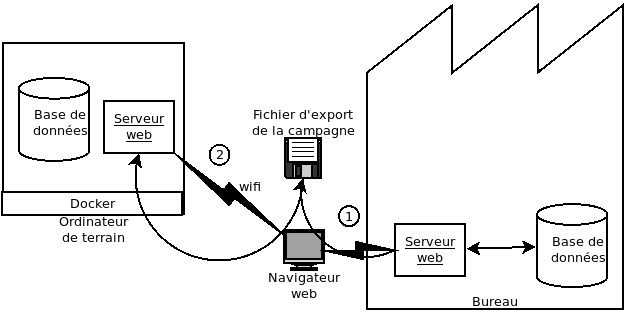
\includegraphics[width=0.8\linewidth]{images/docker_schema_general}
\caption{Schéma général de fonctionnement du mode autonome.}
\label{fig:docker}
\end{figure}

Dans un premier temps, les informations générales sur la campagne sont saisies dans l'application centrale (bureau), ainsi que les informations liées au projet. La campagne est ensuite exportée (modèle d'export : \textit{Description des campagnes}) dans un fichier au format JSON.

Dans un second temps, l'application est installée dans une machine destinée à aller sur le terrain (ordinateur portable Windows, ou couple Raspberry\footnote{Les Raspberry sont des ordinateurs de très petite taille (ils tiennent dans une poche), fonctionnant sans écran ni clavier, destinés à être utilisés un peu partout, et peu chers (quelques dizaines d'euros, moins de 150 euros avec une batterie). Ils fonctionnent avec un système d'exploitation basé sur Linux, et embarquent un émetteur wifi permettant de connecter une tablette, par exemple.} -- tablette Android). 
Un navigateur se connecte au serveur web embarqué qui contient une copie de l'application. À partir de celle-ci, il suffit d'importer le fichier généré précédemment pour récupérer les paramètres du projet et de la campagne.

La saisie s'effectue alors à partir du système autonome. Une fois la campagne terminée, il faut réaliser les opérations dans l'autre sens :  les saisies faites sur le terrain sont exportées au format JSON depuis l'application embarquée (depuis le détail de la campagne, liste des opérations réalisées), puis importées dans l'application centrale.

\section{Installer l'application et la base de données dans un matériel autonome}

L'installation a été prévue pour utiliser un composant particulier, \textit{Docker}, qui permet d'installer n'importe quel système sur n'importe quel autre, tout en gardant le paramétrage particulier du premier.

L'ensemble de la procédure d'installation, à la fois de Docker, de l'application et de la base de données est décrite (en anglais et en français) dans un projet \textit{Github} : \href{https://github.com/Irstea/filo-docker}{https://github.com/Irstea/filo-docker}.
Des instructions particulières concernent l'installation dans un Raspberry, avec l'activation du wifi pour pouvoir connecter une tablette.




%Bibliographie
\backmatter

% Integration de la biblio
% Pour insérer toutes les références : 
%\nocite{*}
% Pour intégrer une référence non citée : 
%\nocite{ref}
\nocite{*}
\bibliography{filo-science}

\end{document}